
We explore five existing estimators of extinction times, discussing each approach's assumptions and reasoning to develop a baseline understanding of the methods available in the literature.

\section{Maximum Likelihood Estimator (MLE)}

We begin by describing maximum likelihood estimation as a method for inferring the extinction time of a species. Under Model \ref{model: no-measurement-error}, assuming uniformity and no measurement error, the Maximum Likelihood Estimator (MLE) is the first order statistic $X_{(1)}$:
\begin{equation}\label{eq:mle}
    \hat\theta_{\text{MLE}} = X_{(1)}
\end{equation}

From a statistical perspective, the MLE procedure is an obvious choice to estimate the extinction time, as one can intuit the most recent fossil as representing the most information about a species' extinction date. However, the incompleteness of the fossil record means that the first and last fossil will never precisely represent the introduction and extinction times of a species. Perhaps for this reason (along with its unrealistic assumptions) maximum likelihood sees limited use in the literature \cite{Ludwig1996, Jaric2016}. Nonetheless, the MLE serves as a straightforward baseline for estimating extinction times.

Consider the likelihood function of the uniform distribution
\[
\mathcal{L}(\theta | \bm{x}) =  \frac{n}{(K - \theta)^{n+1}} > 0 \quad \forall \theta
\]

where $K$ (the upper bound for $X_i$) is a known constant. Differentiating the likelihood, we can show that the derivative is a monotonically increasing function of $\theta$:
\[
\frac{d}{d\theta}\mathcal{L}(\theta | \bm{x} ) = \begin{cases}
    \frac{1}{(K-\theta)^n} & \text{if $X_{(1)} \geq \theta$ and $X_{(n)} \leq K$} \\
    0 & \text{otherwise}
\end{cases}
\]

where $X_{(i)}$ is the $i$\textsuperscript{th} order statistic.

Thus, our maximum likelihood estimator $\hat\theta_{\text{MLE}}$ is the sample minimum $x_{(1)}$. However, this estimator is positively biased as the most recent fossil is always at least as old as the species' extinction date:
\[
    \E[\hat\theta_{\text{MLE}}] = \E[X_{(1)}] = \frac{K}{n+1} + \frac{n}{n+1}\theta
\]

Correcting for this gives us a bias-adjusted MLE:
\begin{equation}\label{eq:ba-mle}
    \hat\theta_{\text{BA-MLE}} = X_{(1)} \frac{n+1}{n} - \frac{K}{n}
\end{equation}

\section{Strauss Estimator}

\citet{Strauss1989} proposed an unbiased estimator based on the maximum likelihood procedure under Model \ref{model: no-measurement-error}, assuming uniformity and no measurement error where both $\theta$ and $K$ are unknown. As before, the MLE for $\theta$ is the first order statistic $X_{(1)}$, and by symmetry the MLE for $K$ is the $n$\textsuperscript{th} order statistic:
\begin{align*}
    \hat\theta_{\text{MLE}} &= X_{(1)} \\
    \hat K_{\text{MLE}} &= X_{(n)}
\end{align*}

Next, to find an unbiased estimate, we take the expectation of both estimators (see appendix for proof):
\begin{align*}
    \E \left[ \hat\theta_{\text{MLE}} \right] &= \frac{K + n\theta}{n+1} \\
    \E \left[ \hat K_{\text{MLE}} \right]  &= \frac{\theta + nb}{n+1}
\end{align*}

Solving the equations simultaneously, $K$ can be eliminated to yields the following:
\[
\E \left( \frac{nX_{(1)} - X_{(n)}}{n-1} \right) = \theta
\]

which is then used to derive the following unbiased Strauss estimator as an alternative to the previously found unbiased MLE:
\begin{equation}\label{eq:strauss}
\hat\theta_{\text{Strauss}} = \frac{n X_{(1)} - X_{(n)}}{n-1}
\end{equation}

The Strauss estimator key distinguishing feature from the MLE is that it does not require assuming a known upper bound $K$. The Strauss estimator is a fairly widely known and well established method, as it has been shown to be optimal under the (unrealistic) assumptions of uniformity and no measurement error \cite{wang_chudzicki_everson_2009}.

\section{McInerny Estimator}

\citet{Mcinerny2006} developed a method for inferring a species' extinction based on previous sightings under Model \ref{model: no-measurement-error}. By assuming uniformity and no measurement error with sighting rate denoted by $\lambda$, the authors proposed a method of estimating the probability $p$ of a fossil\footnote{Note that these papers were concerned with estimating the extinction of species that have been seen relatively recently, but their methods can be similarly applied to a paleontology context where a species is almost certainly already extinct. For the remainder of this section, we will refer to fossils, rather than sightings.} being found as a function of $\lambda$ and the time gap since the last observation:
\[
p = \left( 1 - \lambda \right)^{x_1 - \theta} \quad;\quad \lambda = \frac{n}{K - x_1}
\]

where the recovery rate $\lambda$ is estimated as the number of samples between $K$ and $x_1$ divided by the time interval spanned by the observations. To find the extinction time, consider the extinction time $\theta$ as the terminal record --- that is, the date at which the probability of another fossil being found is less than some threshold probability $p_t$ -- the McInerny estimator $\hat\theta_{\text{MI}}$ is the largest value of $\theta$ that satisfies this condition:
\begin{equation}\label{eqn:mcinerny-estimator}
    \hat\theta_{n; \text{MI}} = \max\left\{ \theta ; \left( 1 - \frac{n}{K - x_1} \right)^{x_1 - \theta} < p_t \right\}
\end{equation}

There are a number of issues with this method for estimating extinctions in the fossil record. First, the authors' approach to modeling $\lambda$ using the interval $[x_1, K]$ positively biases the estimate, as the period of interest should be bounded by $\theta$ instead of $x_1$. This was noted in \citet{Huang2019}, who suggested the following correction: \[ \lambda = \frac{n}{K - \theta} \] This results in the following corrected McInerny estimator: \begin{equation}\label{eqn:mcinerny-bias-corrected-estimator}
    \hat\theta_{n; \text{MI corrected}} = \max\left\{ \theta ; \left( 1 - \frac{n}{K - \theta} \right)^{x_1 - \theta} < p_t \right\}
\end{equation}

Secondly, the selection of the threshold probability $p_t$ is questionable. \citet{Mcinerny2006} proposed setting $p_t = 0.05$ corresponding to a 5\% significance level for a hypothesis test. However, this can result in overestimating how recent a species went extinct, as estimates are based on the 5\textsuperscript{th} percentile. To correct for this, we propose setting $p_t = 0.5$ instead for a median-based estimate, at the risk of making estimates upwards biased and increasing the amount of Monte Carlo error.

Thirdly, a known property of stationary Poisson processes is that the gaps between observations should be exponentially distributed; however, the results from their paper show a geometric distribution with rate $\lambda$ instead. This is because McInerny et al. implicitly assume that time is discretised, an assumption that is not necessarily valid as fossil ages are not often measured in discrete time units.

Finally, McInerny et al.'s method of estimating $\theta$ is dependent on the number of fossil dates --- they note that the number of samples required to achieve a 95\% certainty of extinction may increase beyond what is feasible, making the method less applicable for estimating extinction from fossils. Furthermore, McInerny et al. give every fossil in the time series equal contribution to the estimated extinction time (since sighting rate is calculated using the whole time series).

\section{GRIWM Estimator}

The Gaussian-Resampled Inverse-Weighted McInerny (GRIWM) estimator is an approach based on the previous \citet{Mcinerny2006} method, designed to account for both the influence of sighting rate and radiometric dating error. \citet{Bradshaw2012} assume uniformly distributed fossils and Gaussian-distributed measurement errors for their procedure, which has two main ideas: one, use Gaussian resampling to account for the known radiometric uncertainty associated with each fossil; and two, use the McInerny method to estimate the true extinction time, inversely weighting the contribution of each fossil by their temporal distances to the most recent fossil. They then calculate confidence intervals by generating 10,000 estimates and taking the sample quantile for the interval's endpoints \cite{Bradshaw2012}.

Suppose our observed fossil record $\bm{x} = [x_1, x_2, \dots, x_n]^\top$, with each fossil having a corresponding standard deviation denoted by $\bm{\sigma}=[\sigma_1, \sigma_2, \dots, \sigma_n]^\top$, which represents the variation introduced by radiometric error.

First, resample each fossil according to $X^*_i \sim \mathcal{N}(x_i, \sigma_i^2)$ and sort the resulting set of resamples; denote the resampled fossil record by $\bm{x^*} = [x^*_1, x^*_2, \dots, x^*_n]^\top$.

Next, suppose that the most-recent fossils are more influential on the sighting rate as extinction approaches. Thus, we can apply the McInerny et al. (2006) method to the $k$ most recent fossils, for all $k \in \{2, 3, \dots, n\}$ with threshold probability $p_t$. This results in $n-1$ McInerny estimates: $\hat\theta_{2; \text{MI}}, \hat\theta_{3; \text{MI}}, \dots, \hat\theta_{n; \text{MI}}$. The final estimator can be found by computing a weighted average where the weight $\omega_k$ is the ratio of the interval between the two most recent fossils and the chosen interval:\[
\omega_k = \frac{x^*_{2} - x^*_{1}}{x^*_{k} - x^*_{1}}
\]

Thus, the weighted estimator $\hat\theta_{\text{GRIWM}}$ is calculated as a weighted average over all possible records:\begin{equation}\label{eq:griwm1}
    \hat\theta_{\text{GRIWM}} = \frac{\sum_{k=2}^{n} \omega_k \hat\theta_{k; \text{MI}}}{\sum_{k=2}^{n} \omega_k}
\end{equation}

To calculate confidence intervals, 10,000 estimates of $\hat\theta_{\text{GRIWM}}$ are generated, and the appropriate quantiles are taken. The point estimate of the extinction time is thus found by taking the median of the 10,000 estimates.

The GRIWM estimation method has some notable caveats as a result of the derivation from the McInerny method as well as only accounting for the variation introduced by measurement error and ignoring sampling error. We note that the GRIWM estimate of $\theta$ is positively biased, as the bias is carried over from McInerny's method. This can be corrected for by applying the correction to McInerny's method as per \autoref{eqn:mcinerny-bias-corrected-estimator}, as an implementation using \autoref{eqn:mcinerny-estimator} will result in a positively biased estimator. Another problem carried over from the McInerny method is the choice of the threshold probability $p_t$, which the authors suggested to be 0.05. As was discussed in the previous section, we suggest changing this to 0.5 to produce median-based estimates.

\section{Simulated-Inversion Estimator}

We now describe the simulated-inversion (SI) estimator, a method proposed by \citet{Huang2019}. This method is based on the technique of test-statistic inversion for generating confidence intervals for an unknown parameter $\theta \in \R$ \cite{Carpenter1999}. Before we proceed with the SI estimator, we first introduce test statistic inversion.

Let $\bm{X}$ denote a random vector of $n$ independent and identically distributed random variables from a distribution with CDF $F_X (\cdot; \theta)$. Let $S(\bm{X})$ be a consistent estimator of $\theta$. Denote $\bm{x}$ and $S(\bm{x})$ be a realisation of $\bm{X}$ and $S(\bm{X})$ respectively, and let $\alpha$ be a fixed significance level for the test. Suppose $S$ is stochastically increasing with $\theta$:
\begin{equation}
    \theta_1 < \theta_2 \implies F_S(\theta_1) < F_S(\theta_2) 
\end{equation}

where $F_S(\theta) = \PP_\theta\left\{S(\bm{X}) > S(\bm{x})\right\}$. Then, a central $100(1-\alpha)\%$ confidence interval denoted by $[L, U]$ can be found, where $L$ and $U$ satisfy: \begin{equation}
\begin{aligned}
    \PP_{\theta = L}\left\{S(\bm{X}) > S(\bm{x})\right\} &= \alpha/2 \\
    \PP_{\theta = U}\left\{S(\bm{X}) > S(\bm{x})\right\} &= 1 - \alpha/2
\end{aligned}
\end{equation}

More generally, this method can be used to find the $q$\textsuperscript{th} quantile of $\theta$, $\theta_q$: \begin{equation}\label{eq: inversion}
    \PP_{\theta = \theta_q}\left\{S(\bm{X}) > S(\bm{x})\right\} = q
\end{equation}

This method of constructing confidence intervals exploits the duality between confidence intervals and hypothesis tests. Consider a two-sided test of the null hypothesis $H_0: \theta = \theta_0$ using test statistic $S(\bm{x})$. A $100(1-\alpha)\%$ confidence interval is the set of hypothesised values for $\theta_0$ where the test is not significant at level $\alpha$. The duality refers to the way $\theta_0$ is always in the $100(1-\alpha)\%$ confidence interval if the test is not significant at $\alpha$.

Thus, by inverting the test's acceptance region so that the region is a function of $\theta$ rather than being a function of the test-statistic, a confidence interval may be constructed. This naturally relies on a monotonocity assumption, as inversion is only valid where $\PP_{\theta = \theta}\left\{S(\bm{X}) > S(\bm{x})\right\}$ is stochastically increasing with $\theta$, as illustrated by \autoref{fig:inversion_diagram}.

\begin{figure}[ht]
    \centering
    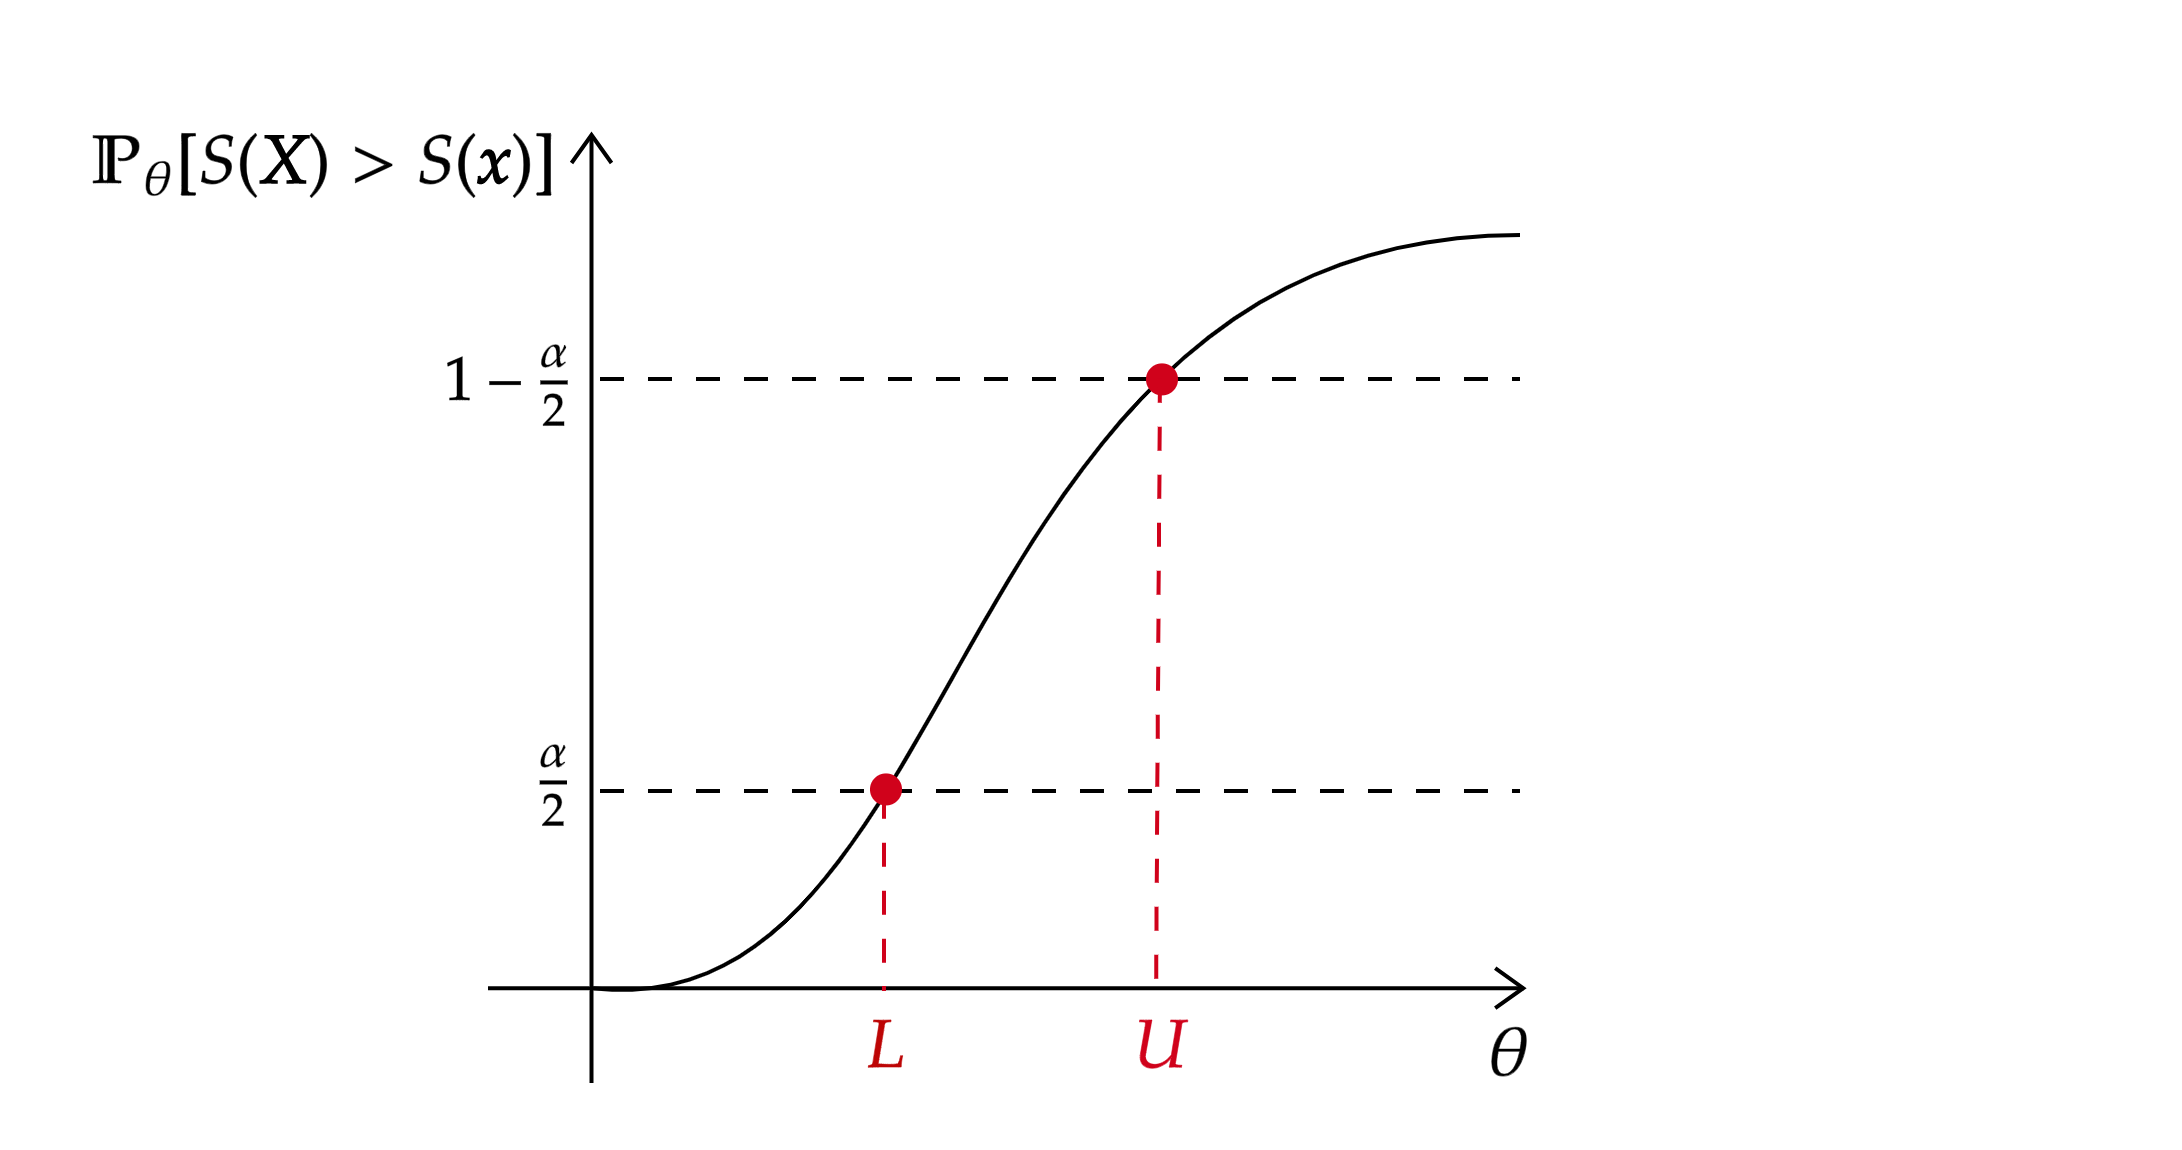
\includegraphics[width=\linewidth]{figures/inversion-diagram.png}
    \caption{The confidence interval - hypothesis test duality. The $100(1-\alpha)\%$ confidence interval for $\theta$, denoted by $[L, U]$, is equivalent to the set of possible values for $\theta$ such that the test statistic $S(\bm{X})$ is in the acceptance region for the null hypothesis. This is only true subject to a stochastically increasing in $\theta$ assumption.}
    \label{fig:inversion_diagram}
\end{figure}

Returning to the simulated-inversion (SI) estimator proposed by \citet{Huang2019}, consider a data generation process following model $M$, which may or may not account for measurement error. The goal is to estimate $\PP_\theta\left\{S(\bm{X}) > S(\bm{x})\right\}$ by simulation, and then construct confidence intervals by inversion. These two steps are described below:

\begin{enumerate}
    \item \textbf{Simulation}: Suppose we have a given dataset $\bm{x} = [x_1, x_2, \dots, x_n]^\top$ and a known set of $r$ potential values for the true extinction time $\bm{\theta} = [\theta_1, \theta_2, \dots, \theta_r]^\top$. Then, for each potential value $\theta_i$, simulate a pseudo dataset $\bm{x}^*_i$ from the model $M$ specified by $\theta_i$ and take a sample statistic $S^*_i$ from the pseudo dataset. Thus, for a given dataset of $n$ observations and a set of $r$ potential values for $\theta$, a set of $r$ simulated statistics $\bm{S}^*$ can be obtained.
    \item \textbf{Inversion}: An estimate for $\PP_\theta\left\{S(\bm{X}) > S(\bm{x})\right\}$ is constructed by regressing the indicator $\mathbbm{1}\left\{ S(\bm{X}^*_i) > S(\bm{x}^*_i) \right\}$ against $\theta_i$ for all $i \in \left\{ 1, \dots, r \right\}$. Finally, $\theta$ can be estimated by inverting the estimated curve.
\end{enumerate}

This method of extinction estimation is very general, as it only requires that the statistic $S(\bm{X})$ is stochastically increasing in $\theta$. It also imposes no other restrictions on the statistic $S(\bm{X})$ used to construct the interval, and imposes no restrictions on the simulation model used to estimate $\PP_\theta\left\{S(\bm{X}) > S(\bm{x})\right\}$, meaning it can be applied regardless of the complexity of the data generation model. Thus, the SI estimator could be used for broader settings beyond the uniform distribution assumption, and could readily account for the presence of measurement errors. For example, Huang suggests the Simulated Inversion - Uniform Gaussian Minimum (SI-UGM) estimator which uses the simulated inversion estimator with the minimum statistic and simulates fossils as uniformly distributed with Gaussian measurement errors \citep{Huang2019}. 

That being said, there are some disadvantages to the SI estimator. Since the true extinction time is unknown, the interval of potential values for $\theta$ must necessarily be wide (and even wider where confidence intervals need to be constructed), which can negatively impact the required computation time for estimating extinction times. In the inversion step, \citet{Huang2019} estimated $\PP_\theta\left\{S(\bm{X}) > S(\bm{x})\right\}$ using a regression method that is not necessarily monotonic, and so this method could be improved by enforcing monotonicity, a conclusion supported by work done by \citet{King2020}.